The data flow diagram from the architectural specification illustrates the comprehensive flow of data within our digital laser harp system. At a high level, the system is structured into three primary layers: the Input Layer, the Control Unit Layer, and the Output Layer.

The Input Layer captures various forms of user interactions and environmental data, including laser interruptions, dials, and buttons for triggering specific actions, and touch screen inputs for more complex settings adjustments. These inputs are collected and transmitted to the Control Unit Layer for processing.

The Control Unit Layer is the core of the system, responsible for managing the logic that governs how inputs are translated into outputs. It houses the Sound Settings, UserSettings, and Sound Multiplexer subsystems. The Sound Settings determine how input adjustments modify sound properties such as pitch and volume. The UserSettings subsystem manages user preferences and configurations, ensuring a personalized experience. The Sound Multiplexer combines the processed inputs to generate the appropriate sound output.

Finally, the Output Layer takes the processed signals from the Control Unit Layer and converts them into audible sound through the Speaker subsystem, as well as visual feedback via the Touchscreen. This layered approach ensures a clear, structured flow of data, from user input to system response, facilitating a seamless interaction between the user and the digital laser harp.
\begin{figure}[h!]
	\centering
 	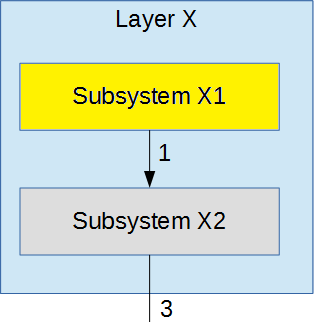
\includegraphics[width=0.90\textwidth]{images/subsystem}
 \caption{System architecture}
\end{figure}
